\documentclass[a4paper, 12pt]{report}
\usepackage[utf8]{inputenc}
\usepackage[english]{babel}
\usepackage{graphicx}
\usepackage{float}
\usepackage{comment}
\usepackage{amsmath}
\usepackage{amsthm}
\theoremstyle{definition}
\newtheorem{definition}{Definition}[section]
\usepackage{listings}
\usepackage{textcomp}
\usepackage{tabu}
\usepackage{xcolor}

\usepackage{setspace}
\onehalfspacing

%\renewcommand*\ttdefault{pcr} 

\usepackage{hyperref}
\hypersetup{
    colorlinks,
    citecolor=black,
    filecolor=black,
    linkcolor=black,
    urlcolor=black
}

\usepackage{titlesec}
\titleformat{\chapter}{\normalfont\huge\bf}{\thechapter}{20pt}{\huge\bf}

\usepackage{fancyhdr}
\pagestyle{fancy}
\fancyhf{}
\rhead{\sc{A. Rahim}}
\lhead{\rightmark}
\cfoot{\thepage}

\renewcommand{\baselinestretch}{1.5} 

%\usepackage[backend=biber,style=numeric,sorting=ynt]{biblatex}
\usepackage[backend=bibtex,style=verbose-trad2]{biblatex}
\bibliography{references.bib}


%\title{UCG Thesis}
%\author{by \\ Abidur Rahim \\ \texttt{abidur@tuta.io}}
%\date{\today}


\begin{document}

%\setlength{\columnsep}{0.3 in}
\begin{titlepage}
    \begin{center}
        \vspace*{1cm}
        
        \sc
        
        \Large
        Which ML Classifier is Best for an IACT?
        
        \vspace{0.5cm}
        
        \normalsize
        Using Five Machine Learning Methods in Mathematica \\ to Classify Monte Carlo Data Generated for the  \\ Major Atmospheric Gamma Imaging Cherenkov Telescopes
        
        %\vspace{0.5cm}
        
        %\large
        
        %An Implementation of Various Unsupervised Machine Learning methods for the Classification of Stars Using Their Corresponding Spectroscopic Data
        \normalsize
        \vspace{1cm}
 
        by \\
        \large
        Abidur Rahim \\
        \normalsize
        (s3140520)
        \vfill
 
        Thesis Submitted in Partial Fulfillment of the \\
        Requirements for the Degree of \\
        Bachelor of Science \\
        %(Free Major in Sciences) \\
        in the Department of \\
        Liberal Arts \& Sciences \\
        University College Groningen
 
        \vspace{0.5cm}
 
        
\includegraphics[width=0.4\textwidth]{im/rug_logo.png}
 
        University of Groningen\\
        Groningen, the Netherlands\\
        August 2019
 
    \end{center}
\end{titlepage}

%\maketitle

\begin{abstract}
    Recent years have been marked by an exponential growth in the amount of digital data, and this is particularly true for the field of Astronomy. Computers can now be taught to interpret large amounts of data and use it to generate possible analytical models. Such implementations can be done in an Imaging Atmospheric Cherenkov Telescope (IACT). In this paper, we work out which of five Machine Learning (ML) methods is best suited for data of the Major Atmospheric Gamma Imaging Cherenkov (MAGIC) Telescopes. To answer this, we construct five different machine learning models using Wolfram Mathematica and compare them. Our findings indicate that the Random Forest algorithm is the ideal candidate for binary classifications of this sort.
    
\bigskip
    
\textbf{Keywords:} Classification, Machine Learning, Mathematica, MAGIC, IACT, Neural Network, Decision Trees, Random Forest, Nearest Neighbors, Logistic Regression, Predictive Modeling.

\end{abstract}


\newpage

\vspace*{1cm}

\textbf{Title of paper:} Which ML classifier is best for an IACT? Using five machine learning methods in Mathematica to classify Monte Carlo data generated for the Major Atmospheric Gamma Imaging Cherenkov Telescopes.

\textbf{Author:} A. A. (Abidur) Rahim

\textbf{Supervisor:} dr. T. C. (Tjeerd) Andringa

\textbf{Co-assessor:} dr. M. A. (Mariet) Hofstee

%\vspace{2cm}

\vfill

\begin{center}
© Abidur Rahim 2019 \\
E-mail: \texttt{\href{mailto:abidur@tuta.io}{abidur@tuta.io}}  \\
University College Groningen \\
Summer 2019
\end{center}

\vspace{1,5cm}


\begin{center}
    This work is licensed under a Creative Commons \\
    Attribution-NonCommercial-ShareAlike 4.0 International License \\
    (\url{https://creativecommons.org/licenses/by-nc-sa/4.0/}) \\
    (CC BY-NC-SA 4.0). \\
\end{center}

\newpage

\chapter*{Acknowledgements}

I would like to thank dr. ir. C. J. G. (Gerco) Onderwater for initially acting as my supervisor, introducing me to the fascinating world of machine learning, and being the inspirational personality that he is. In addition, I would like to thank R. D. (Ralitza) Mondal for being the very best that no one ever was. Lastly, I would like to thank everyone who provided their generous feedback for this paper. The dataset was collected from the University of California, Irvine (UCI) Machine Learning Repository. \autocite{repository} The original owner of the data was R. K. Bock of MAGIC. The dataset was donated to the repository by P. Savicky of the Institute of Computer Science of the Czech Academy of Sciences. The code for the classification models was written in the Wolfram Language on Mathematica version 12.0.0.0. \autocite{wolmat}
\newpage

\tableofcontents

\chapter{Introduction}

This chapter introduces the ties between Machine Learning and Astronomy and sets the ground for our research.

\section{Context}

Recent years have been marked by an exponential growth in the amount of digital data, and this is particularly true for the field of Astronomy. The increasing amounts of data stem from the fact that the number of operating telescopes is increasing, but more so because they are becoming more sensitive and capable of surveying larger and deeper portions of the sky. The Hubble Space Telescope, which was deployed back in 1990, has been transmitting about 120 gigabytes of data every week \autocite{hubblesite}. The Kepler Telescope measures the light from 170,000 stars every 30 minutes. \autocite{keplar} The Sloan Digital Sky Survey SkyServer databases is 818 gigabytes, and the total number of rows exceeds 3.4 billion. \autocite{sdsssite} Moreover, many other telescopes handle similar amounts of data. Considering all the high-tech telescopes that are currently in operation, as well as those that are scheduled to come into operation in the upcoming years, it will be nearly impossible for humans to sort and analyze all the data manually.

Computers can now be taught to interpret large amounts of data and use it to generate possible analytical models. This functionality can become useful when the quantity of data that has to be analyzed becomes too great for humans to sort. With the help of Machine Learning, computers can interpret large amounts of data with the help of algorithms and statistical methods. Only one of the many available methods is the Artificial Neural Network, which comprises of nodes connected in a structure similar to that of the neurons in the human brain. In any case, the model learns from the addition of new data and can continuously improve itself without the need to explicitly program classification rules for the model. The use of Machine Learning has the potential of making data processing much less time consuming and reducing dependence on volunteers to manually work on the data.

%It is possible to use Machine Learning methods to interpret the large amounts of data coming from telescopes. In relation to the data, there are rising concerns as to how and where all the new data will be stored. So it may be a good idea to store just the interpretation of the raw data, since this has the potential of saving storage space. In addition, the raw data of each interstellar object may be classified into predefined groups and just the category of the object can be stored to save additional storage space. In any case, the use of Artificial Intelligence has the potential of making the processing of astronomy data much less time consuming and reducing the dependence on volunteers to manually work on the data.


\section{Machine Learning in Astronomy}

With the advent of the increasing amounts of available data, Astronomers and Astrophysicists have been making an effort to take advantage of the developments of Machine Learning and use of them to interpret said data. The applications of these Machine Learning models are themselves very diverse. Moreover, this phenomenon is by no means a recent development. Artificial Neural Networks had been implemented to classify galaxy spectra back in 1996 \autocite{ANNGalaxySpectra1996}. A good example of a volunteering-based project in Astronomy is the Galaxy Zoo project. \autocite{galzoo} After successful manual classification having been carried out over a number of years, the project resulted in a dataset that could be used to train algorithms to perform the same task automatically, and good progress has been made in relation to the creation of effective classification models.\footnote{See \url{https://www.kaggle.com/c/galaxy-zoo-the-galaxy-challenge/}}

Recent times have seen much more advanced implementations of Artificial Neural Networks and other Machine Learning methods. These include the use of Convolutional Neural Networks. A Convolutional Neural Network has certain properties that make it useful in the analysis of images, so this specific class is of relevance in the field of image analysis. This particular type of Neural Network is concerned with what is called \textit{deep learning}. Its modeling scheme uses \textit{filters} to observe \textit{windows} of image pixels instead of observing each pixel individually. The \textit{filters} generate \textit{features} that can then be used as input variables into the model. This process can be used to interpret the data, but the same algorithm also has the potential of being able to compress the images so that storage space can be saved. A method of data compression such as this can become useful when we consider the quantity of data becoming available. Additionally, these algorithms can be used to increase the quality of images. These networks have recently been used to detect the presence of \textit{gravitational lenses} in images at unprecedented speeds \autocite{Hezaveh2017}. 

\section{Aim of this paper}

With the emergence of such improvements in the field of Machine Learning, it is not usually clear what techniques are best for the interpretation of data in a given situation. Moreover, the type of data that requires processing may also vary. The type of data depends on the specific problem at hand. In this paper, we will aim to answer which machine learning method is best suited for an Imaging Atmospheric Cherenkov Telescope (IACT). The data we will be concerned with was generated for the Major Atmospheric Gamma Imaging Cherenkov (MAGIC) Telescopes located at the Roque de los Muchachos Observatory, La Palma, Canary Islands. MAGIC is a set of two IACTs. The machine learning methods we will be concerned with include Neural Networks, Decision Trees, Random Forests, Nearest Neighbors, and Logistic Regression. For the implementation of the classifiers, we will make use of Wolfram Mathematica.

The dataset includes properties of a detected signal along with a \enquote{class} attribute. The signal detected by an IACT may be caused by a gamma ray -- which the telescope was designed to detect -- or another source that could be a hadron (more specifically baryon) shower. When a signal is observed on this telescope, it is not immediately clear whether the detected signal was in fact the result of a gamma ray. Machine learning methods may viably be used in this case to quickly evaluate if a signal was a gamma ray. Since the signals detected on the telescopes do not come with a class marker, we are compelled to make use of computer generated data to train the models. It will soon be discussed how the data relates to the real world.  Ideally, one would like the classification models to be fast, and most importantly, accurate in its classifications. For this criteria to be fulfilled, one must know \textbf{which machine learning methods are optimal for the classification of gamma rays from IACT data}. This is what we aim to answer in this paper.

It is in our view that the process of automation can lead to the speeding up of advancements in the field of Astronomy. If we know which classification methods work best with a certain type of data, we will be able to automate the process as efficiently as possible. Automation in certain aspects of research will also allow us to focus our energy on more pressing questions. The universe is a big place. It is in fact too big for the human mind to comprehend, let alone analyze extraterrestrial object by extraterrestrial object and phenomenon by phenomenon. Observation is essential in Astronomy, and computers have the potential of making this task faster and more accurate. With that said, we hope this research contributes to our understanding of the cosmos and our place in it.

\chapter{Dataset}

This chapter serves to describe the properties of the data that was used for the creation of the classification models. It also explains what programs were used to generate the data, as well as why we needed to use this simulated data to train our models in the first place.

\section{Cherenkov radiation}

The Earth's atmosphere is not completely transparent to much of the electromagnetic radiation that it receives from space. As such, telescopes detecting certain wavelengths of light must be deployed into space so that photons of that particular wavelength can be observed optimally. Only light in the visible and radio bands of the electromagnetic spectrum are easily detected from the ground surface. This phenomenon is better described in Figure 2.1 \autocite{opacity}. Space telescopes, however, are much more costly than ground-based telescopes. In addition, the size of the effective photon collection area is restricted in the case of space telescopes. Consequently, it also becomes difficult to detect relatively low energy photons. Gamma rays arriving from outer space also usually get absorbed in the upper atmosphere. Fortunately, there are indirect means through which these gamma rays can be detected.

\begin{figure}[h!]
  \centering
  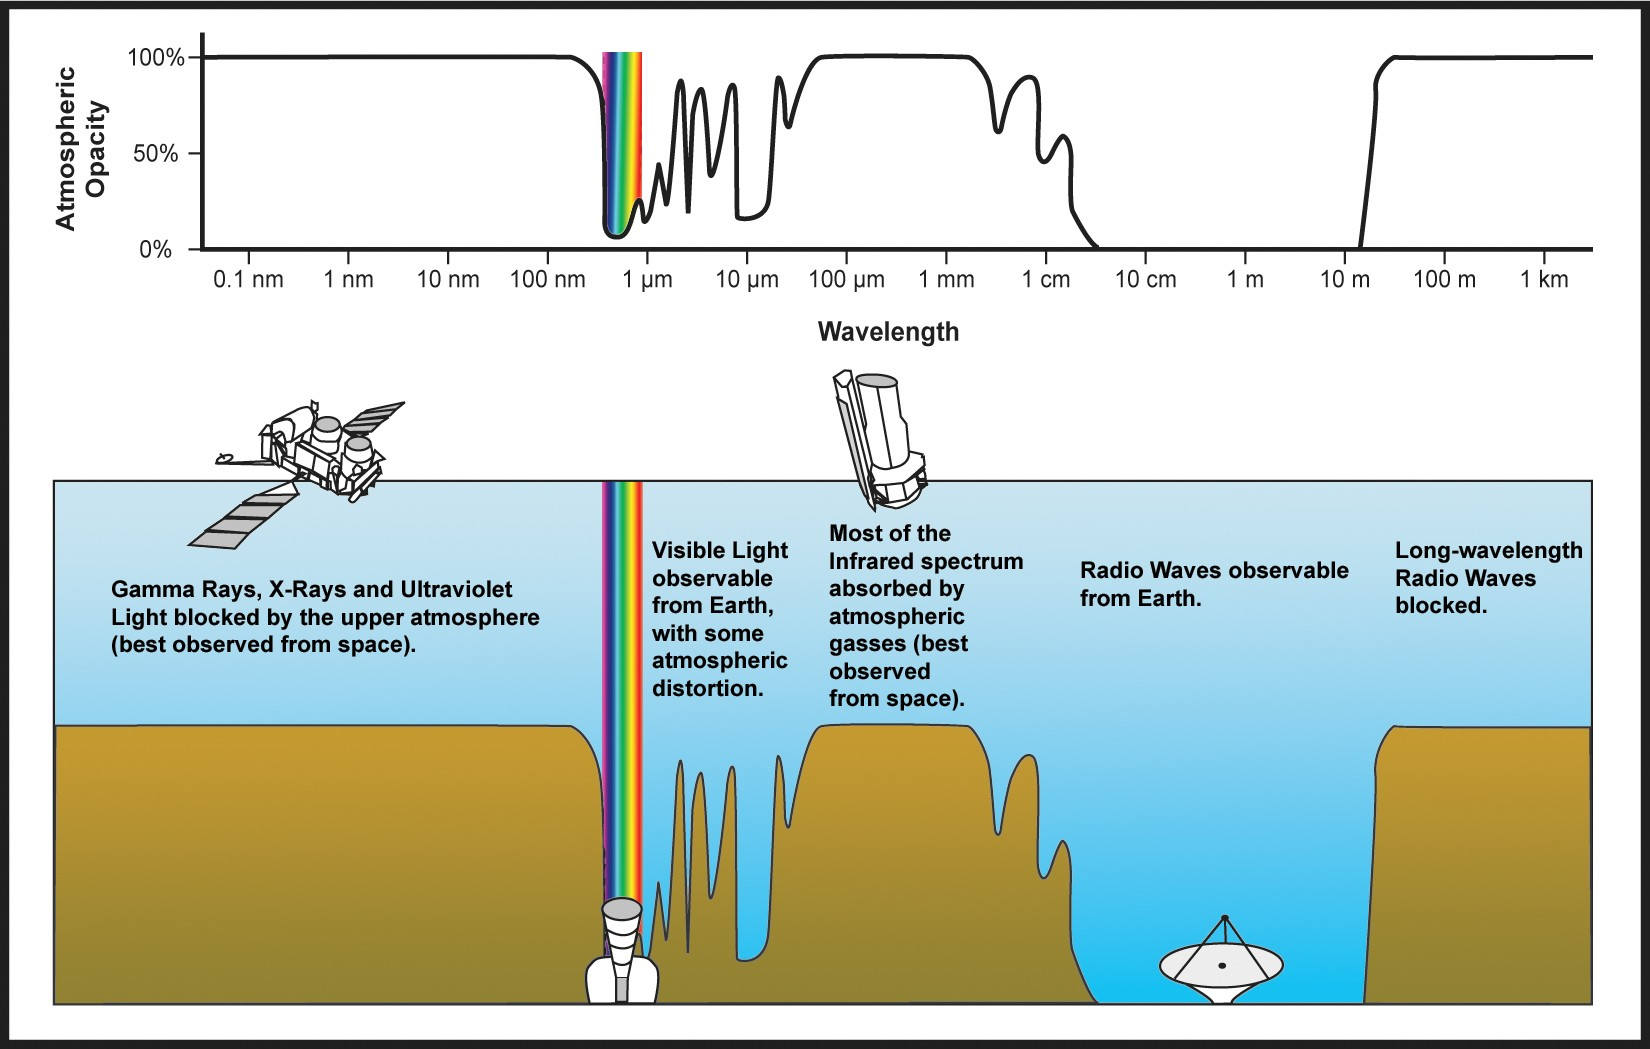
\includegraphics[scale=0.95]{im/atmosphericopacity.jpg}
  \caption{Atmospheric opacity across the electromagnetic spectra.}
  \label{fig:atmopacity}
\end{figure}

Cherenkov radiation allows the indirect detection of high energy gamma rays. When certain conditions are met, a photon can create an electron and its corresponding antiparticle pair, i.e. a positron. A high energy gamma ray or cosmic ray can cause this process to occur in the atmosphere. The emitted particles can have a velocity greater than that of light in the medium (but not greater than the velocity of light in a vacuum, of course). When the new charged particle (usually the electron since the positron tends to get annihilated quickly) moves through an electrically polarizable medium such as the Earth's atmosphere, it creates what is referred to as Cherenkov radiation. This radiation is a sonic boom of light in the shape of a cone (or ring, depending on viewing angle), created by the electron moving at speeds greater than light in air, and then decelerating. This radiation usually lies between the visible and ultraviolet wavelength ranges, and is thus observed as being blue. Observing this radiation can allow us to infer the properties of the ray that caused the process to occur in the first place.

For the particles that reach the required velocity to produce Cherenkov radiation, where $v$ is the velocity of the particle, $c$ is the speed of light in a vacuum, and $n$ is the index of refraction, the following condition holds:
\begin{equation}
    nv/c = n\beta > 1
\end{equation}

The geometry of Cherenkov radiation is shown in Figure 2.2. \autocite{cherenkovcom} The emission angle, $\theta_c$, with respect to the velocity of the charged particle is given by the equation:

\begin{equation}
    \cos{\theta_c} = \frac{1}{\beta n}
\end{equation}

\begin{figure}[h!]
    \centering
    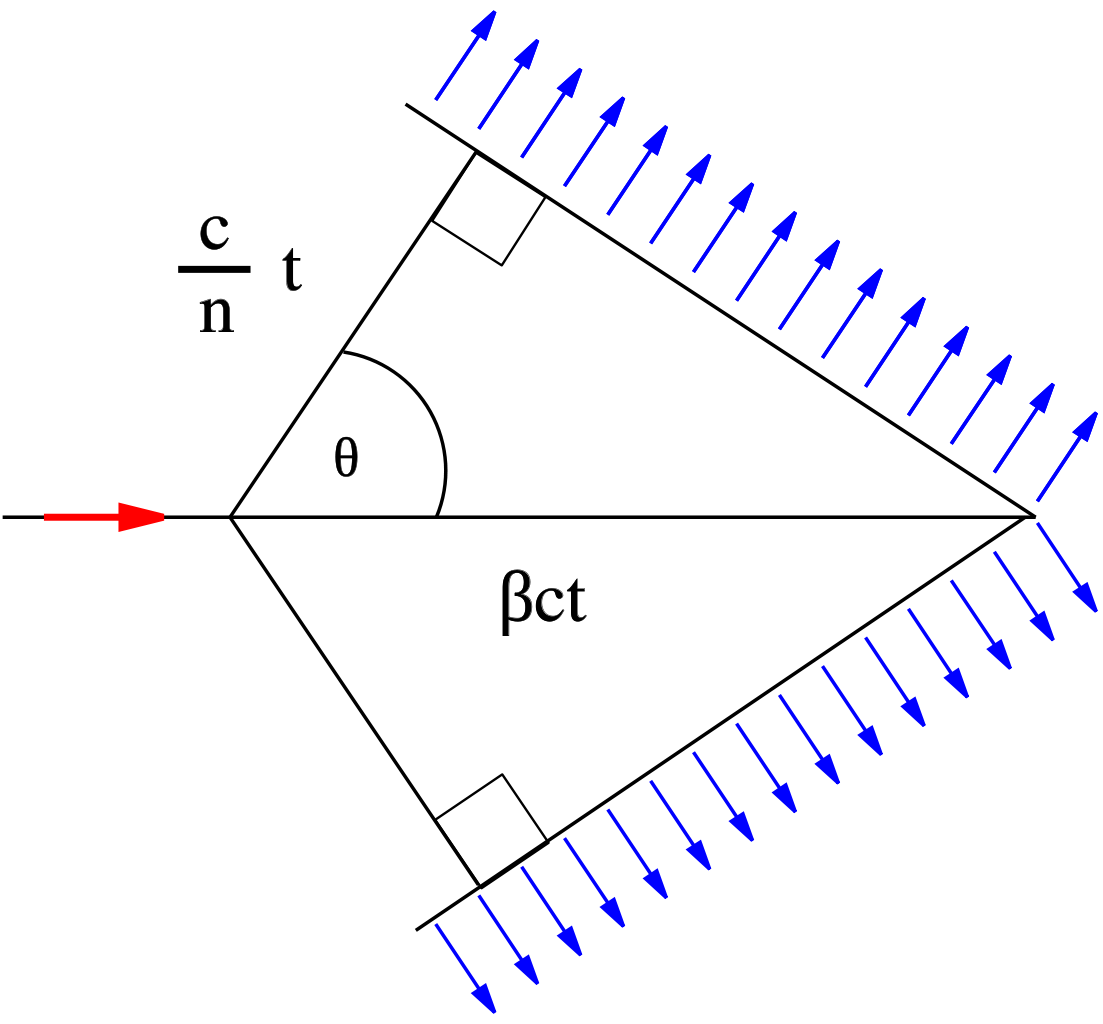
\includegraphics[width=0.4\textwidth]{im/cherenkovcom.png}
    \caption{The geometry of the Cherenkov radiation. Here, $v$ is the velocity of the particle (red arrow), $\beta = v/c$, and $n$ is the refractive index of the medium. The blue arrows shows the direction of propagation of the radiation.}
    \label{fig:cherenkovcom}
\end{figure}

Given the fine structure constant $\alpha$, the number of photons, $N_c$, emitted per path length $s$ at an angle $\theta_c$ is calculated over the wavelength integral across which the Cherenkov detector is sensitive \autocite{corsika_phys}:
\begin{equation}
    \frac{dN_c}{ds} = 2\pi \alpha \int \frac{\sin^2\theta_c}{\lambda^2} d\lambda
\end{equation}

Finally, the Frank-Tamm equation governs the \textit{frequency spectrum} of this phenomenon:
\begin{equation}
    \frac{d^2E}{dx d\omega}=\frac{q^2}{4\pi}\mu(\omega)\omega \left(1-\frac{c^2}{v^2n^2(\omega)}\right)
\end{equation}

Here, $\beta = \frac{v}{c} > \frac{1}{n(\omega)}$, $q$ and $v$ are the electric charge and speed of the particle respectively, $E$ is the energy, and $\mu(\omega)$ and $n(\omega)$ are the permeability and index of refraction of the medium respectively.

The above relations are what determine the characteristics of the detected Cherenkov signal.

\section{Generation of data}

The use of computational methods is by no means a new phenomenon in Astronomy. This section underlines some of the strategies used to generate the data we are concerned with.

\subsection{Monte Carlo method}

In Statistics, the \textit{Law of Large Numbers} states that: \enquote{As the number of identically distributed, randomly generated variables increases, their sample mean (average) approaches their theoretical mean \autocite{largenumbers}.} This law is the basis of the Monte Carlo method, which was named after the famous casino in Monaco. The Monte Carlo method is extremely useful because it allows deterministic problems to be solved using randomness and probability. Moreover, in cases such as ours where there are many coupled degrees of freedom for the parameters governing the system, the Monte Carlo method can serve as a useful modeling tool.

In general, all Monte Carlo methods involve the following steps. Firstly, a domain is assigned over which inputs are derived from a probability distribution. In this regard, a source of uniformly distributed pseudo-random numbers is essential. Fortunately, many methods are now available to do so. Finally, the randomly generated inputs undergo a deterministic computation, after which the results are aggregated. Since the advent of this method, applications have been found in a broad spectrum of physical and mathematical problems ranging from galaxy evolution modeling to financial risk analysis.

Although Monte Carlo methods use probability distributions and randomness in their execution, the models usually come very close to the real value, as stated by the Law of Large Numbers. The accuracy of predictions depends to a large extent on the computational time available. However, rapid technological progress will surely make the predictions even better. This means that Monte Carlo methods will remain useful and applicable for real world scenarios. One such program that uses the Monte Carlo method is CORSIKA, which will be discussed next. CORSIKA was used to generate the dataset.

\subsection{CORSIKA}

CORSIKA (COsmic Ray SImulations for KAscade) is a program for detailed simulation of extensive air showers initiated by high energy cosmic ray particles \autocite{heck_pierog_2018}. It was initially developed in order to perform simulations for the KASCADE experiment at Karlsruhe, Germany \autocite{kascade}. It is mentioned in the documentation that protons, light nuclei up to iron, photons, and many other particles may be treated as primaries. A detailed description of the program can be found in the Documentation section of the CORSIKA website \autocite{corsika_phys}. Over time, CORSIKA has become an important program for gamma ray, cosmic ray, and neutrino Astronomy. The purpose of CORSIKA is to perform a “particle transport with stochastic and continuous processes” \autocite{nextgencorsika}.

The creators of the dataset ran CORSIKA with parameters allowing the observation of events with energies down to below 50 GeV. As a reference, IACTs usually detect events of relatively high energies in the range of around 50 GeV to 50 TeV. The dataset was meant for use with the MAGIC (Major Atmospheric Gamma Imaging Cherenkov) telescopes project. MAGIC is one of four Imaging Atmospheric Cherenkov Telescopes operating as of the writing of this paper. In CORSIKA, the refractive index $n$ is approximated by ignoring the wavelength dependence of $n$ and using the local density $\rho(h)$ \autocite{weast_1986}:
\begin{equation}
    n = 1 + 0.000283 \times \frac{\rho(h)}{\rho(0)}
\end{equation}

\begin{center}
    \begin{table}[p!]
        \renewcommand{\arraystretch}{1.5}
        \begin{tabular}{| c | c | p{9cm} |}
        \hline
        \textbf{Attribute} & \textbf{Unit} & \textbf{Description} \\
        \hline
            fLength & mm & Major axis of ellipse \\
            fWidth & mm & Minor axis of ellipse \\
            fSize & [$N_c$] & 10-log of sum of content of all pixels \\
            fConc & [ratio] & Ratio of sum of two highest pixels over fSize \\
            fConc1 & [ratio] & Ratio of highest pixel over fSize\\
            fAsym & mm & Distance from highest pixel to center, projected onto major axis \\
            fM3Long & mm & 3rd root of third moment along major axis \\
            fM3Trans & mm & 3rd root of third moment along minor axis \\
            fAlpha & deg & Angle of major axis with vector to origin \\
            fDist & mm & Distance from origin to center of ellipse \\
            class & [g/h] & Gamma (signal), hadron (background) \\
        \hline
        \end{tabular}
        \caption{\label{tab:dataset} Attributes of the dataset along with a description.}
    \end{table}
\end{center}

\begin{figure}[t!]
  \centering
  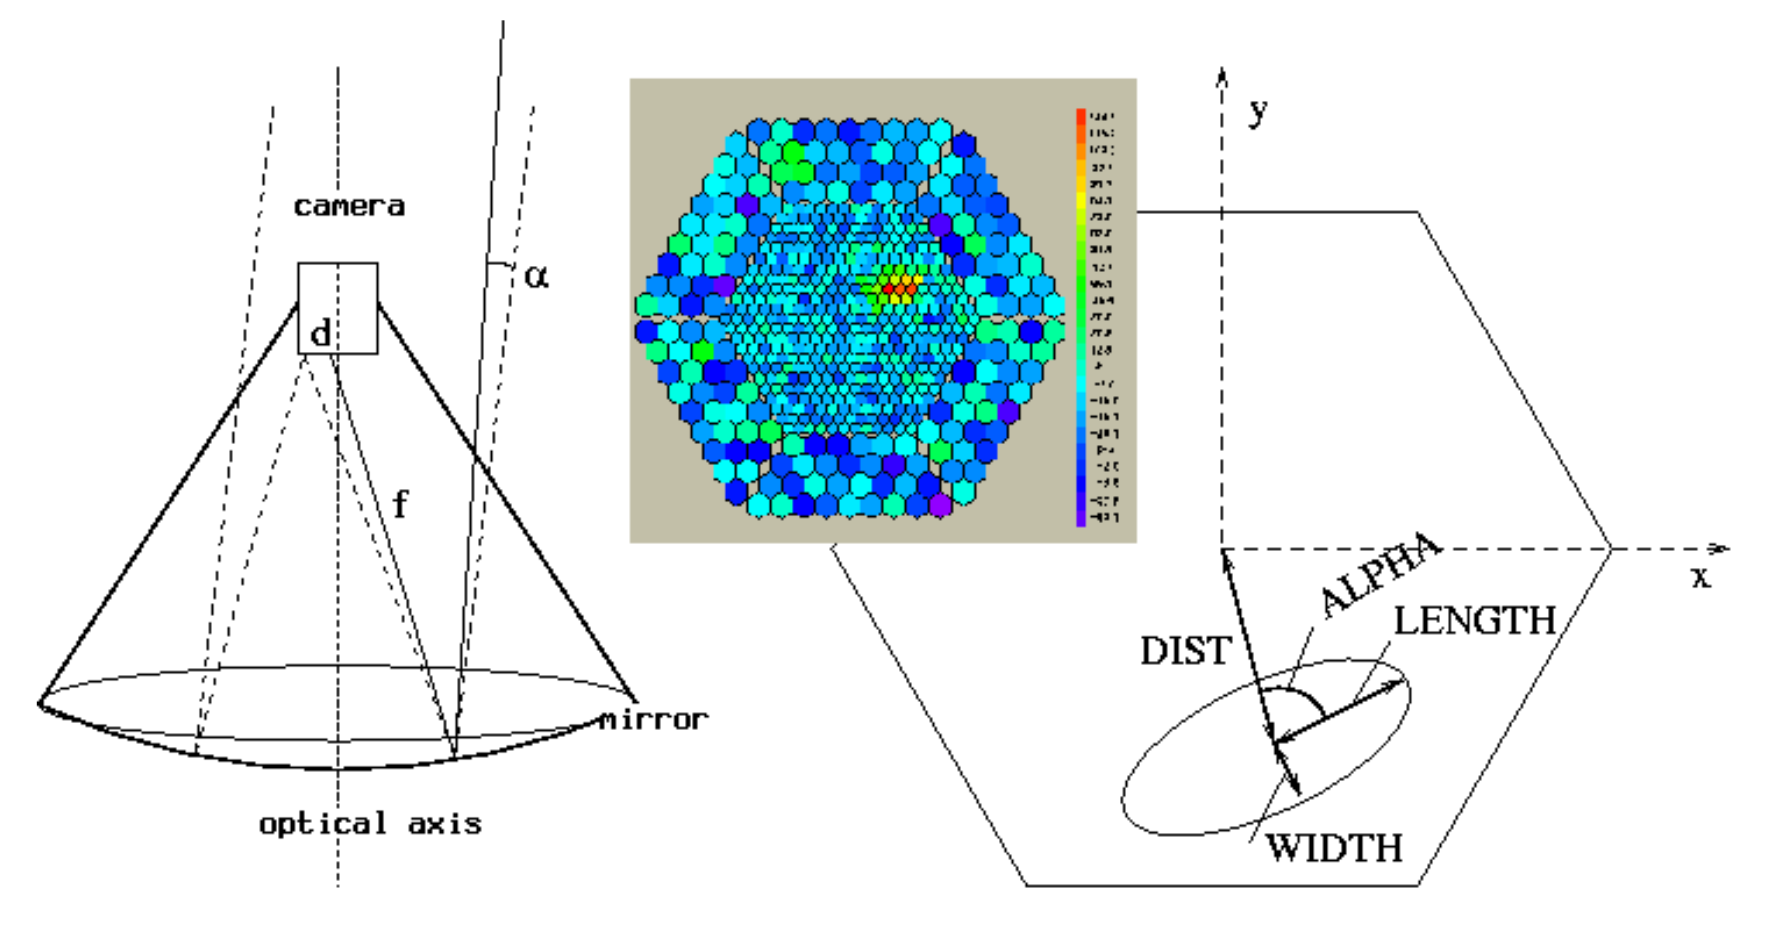
\includegraphics[scale=0.27]{im/telescope.PNG}
  \caption{Cherenkov telescope: sketch and image parameters, and a simulated event in MAGIC (inset).}
  \label{fig:telescope}
\end{figure}

\section{What is being detected?}

The dataset was collected from the UCI Machine Learning Repository \autocite{repository}. The file can be found here \autocite{dataset}. The dataset was generated through the aforementioned processes. From our above understanding, it can be presumed that the dataset we are concerned with accurately mimics a real world scenario, and that the models we are to create will fulfill an useful purpose in that they may later be used to classify real data observed from the telescope. A description of the attributes of the dataset is given in Table 2.1. The relevant parameters correspond to the telescope as shown in Figure 2.3 \autocite{bock_wittek_2003}.

When we create our models, we will allow the program to decide for itself what parameters should be used for classification. Regardless, the dataset information \autocite{dataset} gives us hints as to how the signal may be distinguished from noise, i.e. how gamma ray showers can be differentiated from hadron showers. It proposes that the Hillas parameters of the ellipse, the asymmetry of energy depositions along the major axis, the extent of the cluster in the image plane, and the total sum of depositions can all be used as suitable parameters to carry out classification.

In the real world, we will not know whether the detected signal is from a gamma ray or not. The training of the models, however, requires that the model sees examples of signals and noise so that they can learn to distinguish between them. This is why the data we have used to train and test the models was generated from a computer program. The dataset was generated to closely represent what is actually observed in Imaging Atmospheric Cherenkov Telescopes. It is important that we create ideal models so that we are able to tell with confidence that we know what we have detected. The models we will construct are generic in the sense that the same code can be used to create classification models from a different set of data. Here, we will base our interest in which modeling methods are best suited for classification given the properties of our dataset. With that said, we will now move our focus to the classification methods to be used.

\chapter{Classification Methods}

Over the course of recent years, a number of classification methods have been developed in order to classify and interpret data. For the purpose of this paper, the \texttt{Method} parameter of Mathematica's \texttt{Classify} function was changed to the desired classification method. After these five models are constructed, they can be compared in order to deduce which worked best. This chapter describes the classification methods used.

\section{Training the models}

A number of steps have to be carried out in order to generate a classification model. Initially, the complete sample dataset has to be randomly partitioned into a \textit{training set} and a \textit{test set} (also known as a \textit{validation set}). The training set is used by the model to learn how to classify the data. If a model is taught using all of the available data, we will not be able to test it to see how well it performs. Use of data that the model has seen beforehand is not ideal since the model may recognize that iteration of the data and remember its corresponding class. As such, the model may \textit{overfit} the data. This means that it will be accurate with the data it was trained with, but have a low prediction accuracy for new data. Conversely, accuracy is lowered when the models \textit{underfit} the data. Obviously, we want to avoid both these cases.

\section{Artificial Neural Network}

An Artificial Neural Network (ANN) is an interconnected assembly of simple processing elements, \textit{units} or \textit{nodes}, whose functionality is loosely based on the animal neuron. The processing ability of the network is stored in the interunit connection strengths, or \textit{weights}, obtained by a process of adaptation to, or \textit{learning} from, a set of training patterns. \autocite{gurney_2014} An example of an artificial neural network is given in Figure 3.1 \autocite{NNarchitecture}.

\begin{figure}[h!]
  \centering
  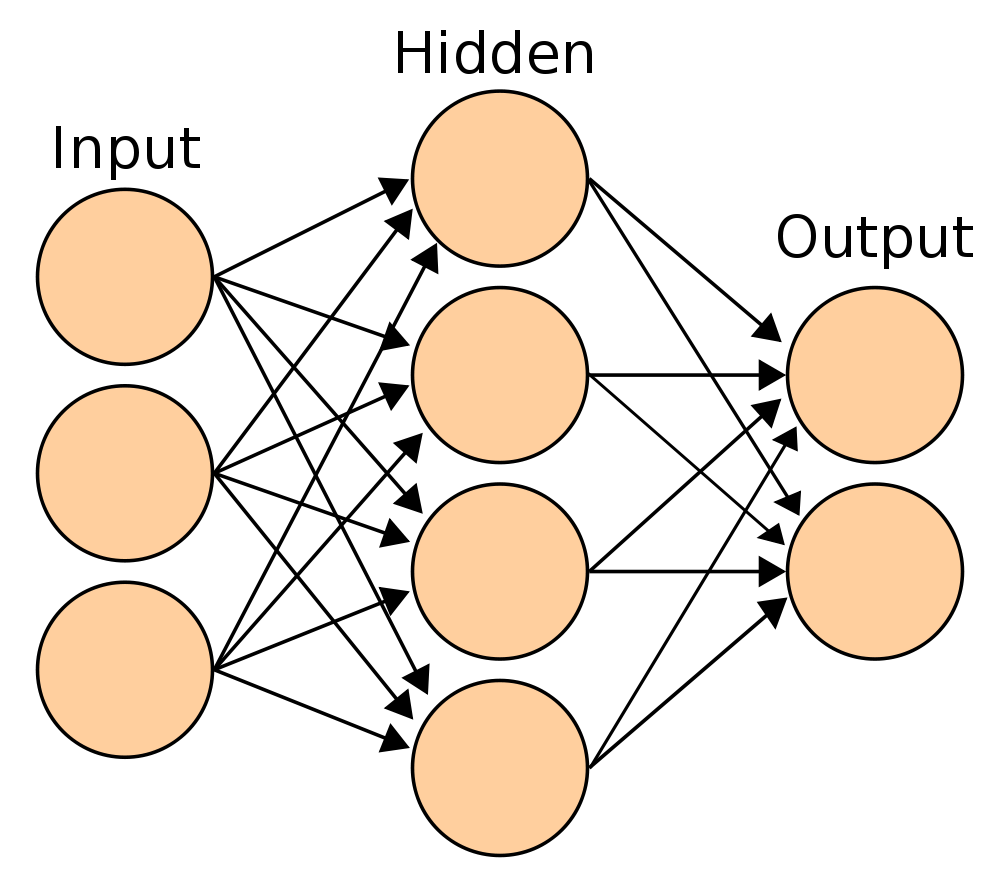
\includegraphics[width=0.5\linewidth]{im/ANN.png}
  \caption{An Artificial Neural Network with one Hidden Layer.}
  \label{fig:ANN1}
\end{figure}

Consider any one of the nodes in the \enquote{hidden} layer. Notice that each node in this layer is connected to every node in the input layer. Signals travel from the nodes of the input layer into a hidden layer. Let these signals be called $x_i$. Each connection from a node in the input layer to a node in the hidden layer is associated with a weight factor, $w_i$. Each node in the hidden layer then processes all the signals it receives to calculate the activation, $a$. Each signal $x_i$ is multiplied with the associated weight $w_i$ and this is done for all the connections that the node in the hidden layer receives from the input layer. The activation $a$ (which is analogous to the action potential) is thus the sum of these products, given by the equation:
\begin{equation}
a = w_1x_1 + w_2x_2 + \dots + w_nx_n = \sum_{i = 1}^n w_ix_i
\end{equation}

If the activation $a$ reaches a certain threshold value $\theta$, the node will activate and send out a signal to the next layer. This signal is denoted as output $y$ of the node and will equal one just in the case that the threshold is reached:
\begin{equation}
y = 
\begin{cases}
  1, & \text{if } a \geq \theta,\\
  0, & \text{if } a < \theta.
\end{cases}
\end{equation}

However, the signal generated may not naturally be distinctly binary. The strength of the signal may vary, as in the case of biological neurons. To represent this, the \textit{sigma function} is used on the activation. The quantity $\rho$ determines the exact shape of the function and is sometimes chosen to be equal one. Figure 3.2 shows this function along with its derivative. It is given by the equation:
\begin{equation}
    y = \sigma(a) = \frac{1}{1+e^{-(a-\theta)/\rho}}
\end{equation}

\begin{figure}[h!]
  \centering
  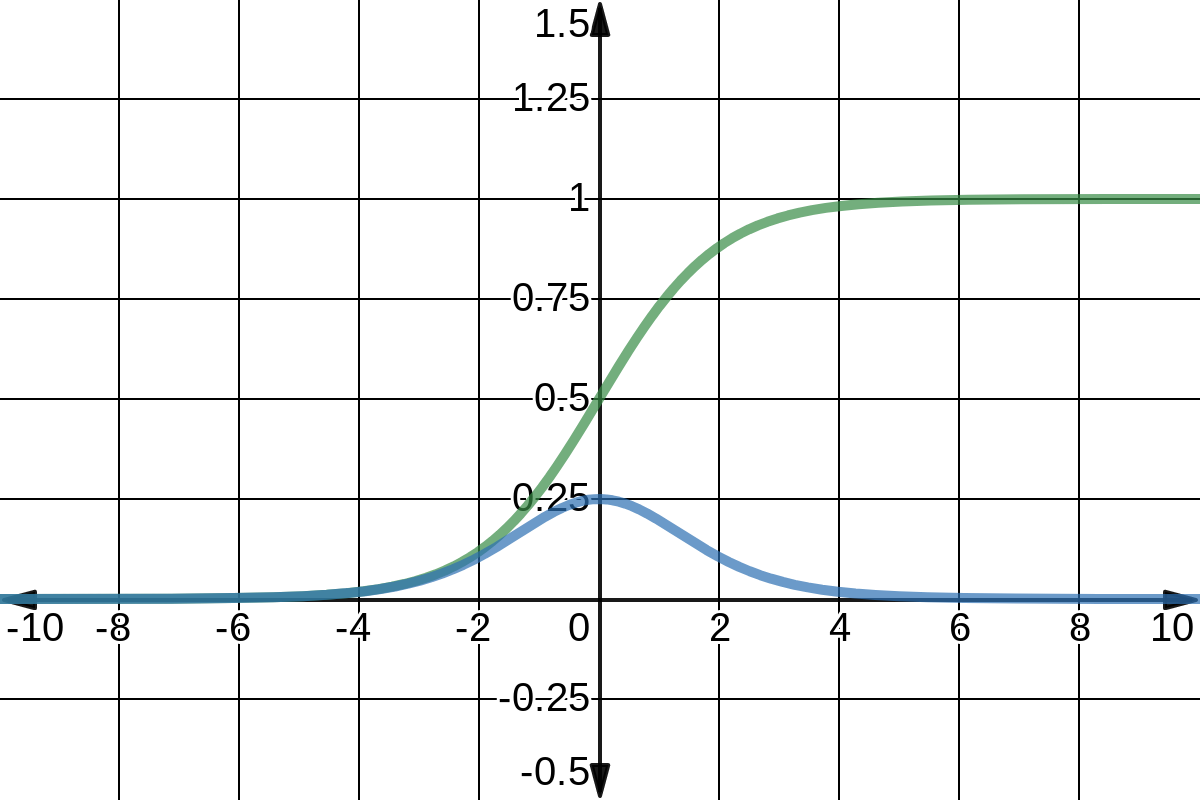
\includegraphics[width=0.7\linewidth]{im/sigmoid.png}
  \caption{A sigmoid function (green) with $\rho = 1$ and its derivative (blue).}
  \label{fig:NNsig}
\end{figure}

The same process occurs in all the nodes of the network. A neural network consists of stacked layers and may have multiple hidden layers. Regardless of how many nodes or layers the network has, information is processed layer by layer from the input layer to the output layer. The network is fed inputs and expected outputs. The \textit{training} of the network basically involves the adjustment of the weights, $w_i$, such that the network returns the desired output. For this the training set is used. The aim of the training is to minimize a \textit{loss function} which gives the error. The total error $E$ of the network is a function of the sum of the errors, $e^{p}$, for each training pattern $p$. Note that $p$ is a step or epoch, and not a power. $E$ is a function of the target value $t^{p}$ and activation $a^{p}$ over each training pattern $p$:

\begin{equation}
    E = \frac{1}{N} \sum_{p=1}^N e^{p}= \frac{1}{2N} \sum_{p=1}^N  (t^{p} - a^{p})^2
\end{equation}

The neural network is trained to minimize the error using the \textit{gradient descent} method, where $\alpha$ is the \textit{learning rate}. This is synonymous to finding the minimum of a function using its derivative:

\begin{equation}
    \Delta x_i = - \alpha \frac{\partial y}{\partial x_i} \implies \Delta w_i = - \alpha \frac{\partial E}{\partial w_i}
\end{equation}

The true gradient $\partial E / \partial w_i$ can be approximated using:

\begin{equation}
    \frac{\partial e^p}{\partial w_i} = -(t^p - a^p) x^p_i
\end{equation}

It can then be derived that the change in weight, $\Delta w_i$, for each epoch, $p$, is determined by the \textit{learning rule}, given by the equation:
\begin{equation}
    \Delta w_i = \alpha \sigma '(a) (t^p -y^p) x^p_i
\end{equation}

There are many techniques that can be incorporated into the network in order to allow it to solve more complex problems. These include the addition of more hidden layers, changing the number of nodes in a layer, and using methods such as \textit{backpropagation}. Regardless, the basic working of the networks remains the same in that weights are adjusted in order to generate the desired outputs. Although seemingly complex computationally, neural networks behave in a way similar to that of the brains of animals. This allows them to be used for a wide range of purposes and makes them capable of modeling nonlinear dynamic systems. Thus this machine learning method has gained popularity and has increased in both complexity and application. However, the resulting weight values are difficult for humans to interpret.

\section{Decision Trees}

A Decision Tree, sometimes referred to as a Classification and Regression Tree (CART) model, is an algorithm composed of conditional control statements arranged in the shape of a hierarchical flowchart or tree. The nodes of the decision tree are usually traversed from top to bottom. In our case, each \textit{internal node} of the tree represents a test on an attribute based on its value, each connecting \textit{branch} or \textit{edge} represents the outcome of the test and connects it to the subsequent node, and each \textit{leaf} represents a terminal node that gives us an output class (in our case a label but this could also be a distribution). An example of a simple decision tree is given in Figure 3.3 \autocite{introdatamining}.

\begin{figure}[h!]
  \centering
  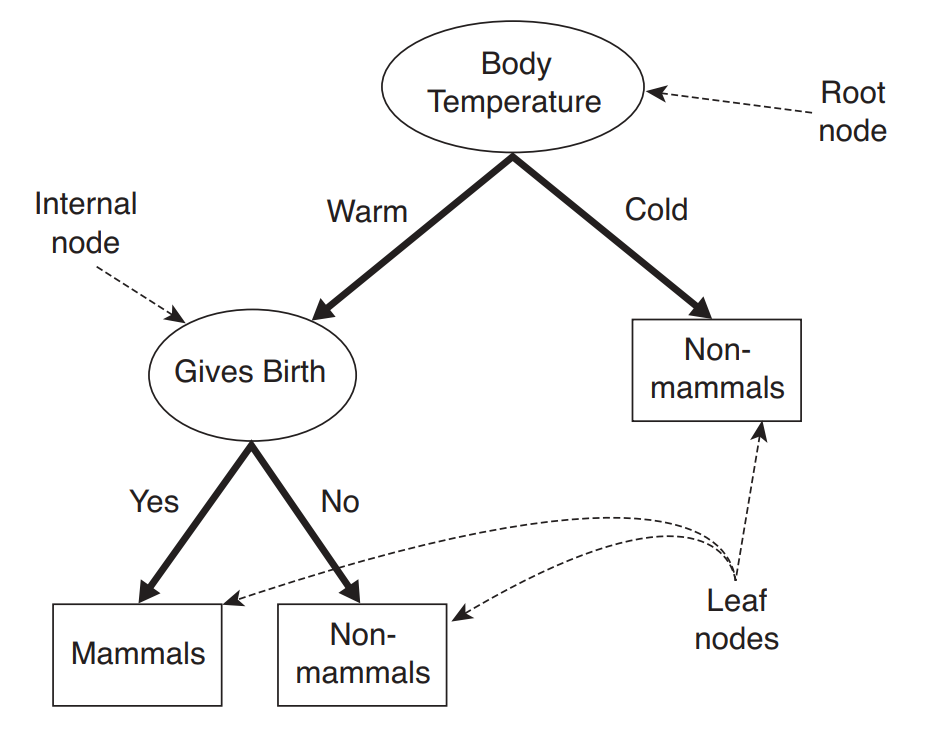
\includegraphics[width=0.7\linewidth]{im/decisiontreeex.png}
  \caption{A decision tree for the classification of mammals.}
  \label{fig:DT1}
\end{figure}

In our dataset, the output variable we are concerned with is categorical and thus the tree should be constructed through what is called \textit{binary recursive partitioning}. As the name suggests, this involves finding the clusters formed by the data and repeatedly using nodes to separate the data into two subsets for each node iteration. This process is repeated until both branches of a node represent the same class, i.e. until the leaves are \enquote{pure}. This classification method is relatively easy to comprehend due to its use of conditional statements in order to create partitions. Thus this method is useful when it is important that one understands how the classification is carried out. Trees with fewer levels are especially easy to understand as the decision process is similar to that of a human being. This implies that classification is relatively fast, especially since insignificant attributes may be ignored altogether.

A significant disadvantage of decision trees is that they are prone to \textit{overfitting}. \autocite{storey_2018} In cases where the properties that distinguish the classes are not simple, this becomes a problem. An important reason as to why this happens is from the fact that the decision boundary is always parallel to the values on the attribute axis \autocite{chakure_2019}. An ideal decision tree makes use of attributes that result in the largest \textit{information gain}. This is sometimes difficult since decision trees are greatly dependent on the training set they are provided. Overfitting can be reduced by intentionally limiting the depth of the tree. Another means of reducing overfitting is by the use of a Random Forest classifier, which comprises of an ensemble of parallel decision trees. This is described next.

\section{Random Forest}

Breiman originally defined the Random Forest classifier as follows:

\theoremstyle{definition}
\begin{definition}{\textbf{Random Forest:}}
A random forest is a classifier consisting of a collection of tree-structured classifiers $\{h(\textbf{x}, \Theta_k ), k = 1, \dots\}$ where the $\{\Theta_k\}$ are independent identically distributed random vectors and each tree casts a unit vote for the most popular class at input \textbf{x}. \autocite{breiman2001random}
\end{definition}

As one may be able to infer from the name, a random forest is composed of a collection of decision trees, the predictions of which are averaged to provide a final output. As with decision trees, the algorithm can be used for both classification and regression. A simplified version of a random forest algorithm is shown in Figure 3.4.\autocite{RandomForestArch} 

\begin{figure}[h!]
  \centering
  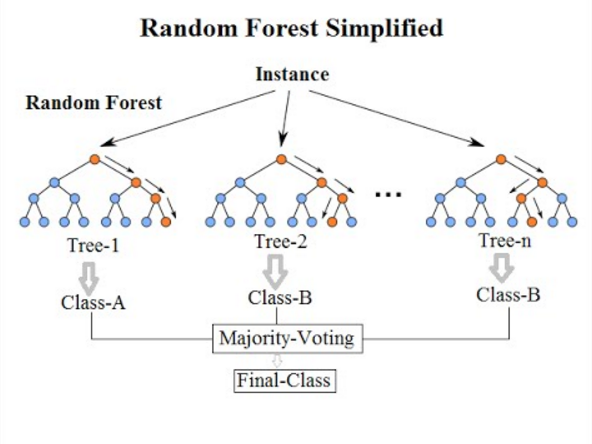
\includegraphics[width=0.75\linewidth]{im/Random_forest_diagram_complete.png}
  \caption{A simplified Random Forest algorithm.}
  \label{fig:RF1}
\end{figure}

Random forest is a parallel, ensemble learning method. This means that it is a combination of a multitude of algorithms, in this case decision trees. Each tree by itself is a \enquote{weak} classifier and makes predictions independently from one another. A single tree in itself is prone to overfitting. However, this is overcome in a random forest model with the use of what is called a \textit{bootstrap aggregating algorithm}. This process is also referred to as \enquote{bagging}. Bagging refers to the process of using a random subset of the features in a random subset of the training data in order to train each individual tree in the ensemble. In the case of a classification example, the final prediction of the forest is the most common class label predicted by the combination of all the trees in the ensemble. Thus the \enquote{winner takes all}. For the ensemble model, the forest output probability is given by:
\begin{equation}
    p(c|\textbf{v}) = \frac{1}{T} \sum_t^T p_t (c | \textbf{v})
\end{equation}

A primary disadvantage of random forests is that the results are not easily interpretable: that is, if you would like to draw conclusions about the meaning of the classification model, random forests may not be the best choice. \autocite{vanderplas_2016} However, the models generated from this method greatly decrease both variance and bias due to its ensemble architecture, and this usually makes them relatively good predictors. 

The Gini Index and Entropy can both be used to give us a measure of the \enquote{node impurity} where $p(c_i)$ is the probability of class $c_i$ being at a node:
\begin{equation}
    \text{Gini} = 1 - \sum_{i=1}^n p^2(c_i) 
\end{equation}
\begin{equation}
    \text{Entropy} = \sum_{i=1}^n - p(c_i)\log_2\left(p(c_i)\right) 
\end{equation}

\section{Nearest Neighbors}

A $k$-Nearest Neighbors (\textit{k}NN) algorithm is a classification (and regression) method wherein the model guesses the class (or value) of a new instance by taking the modal class (or mean) of the $k$ closest instances to the new instance. The \textit{k}NN algorithm is a type of instance-based learning, meaning that rather than creating explicit rules for classification, it compares new instances to the training instances stored in its memory. In general, $k$ must not be a multiple of the number of classes because that could cause multiple modes to manifest. Three example \textit{k}NNs are shown in Figure 3.5 \autocite{introdatamining}.

\begin{figure}[h!]
  \centering
  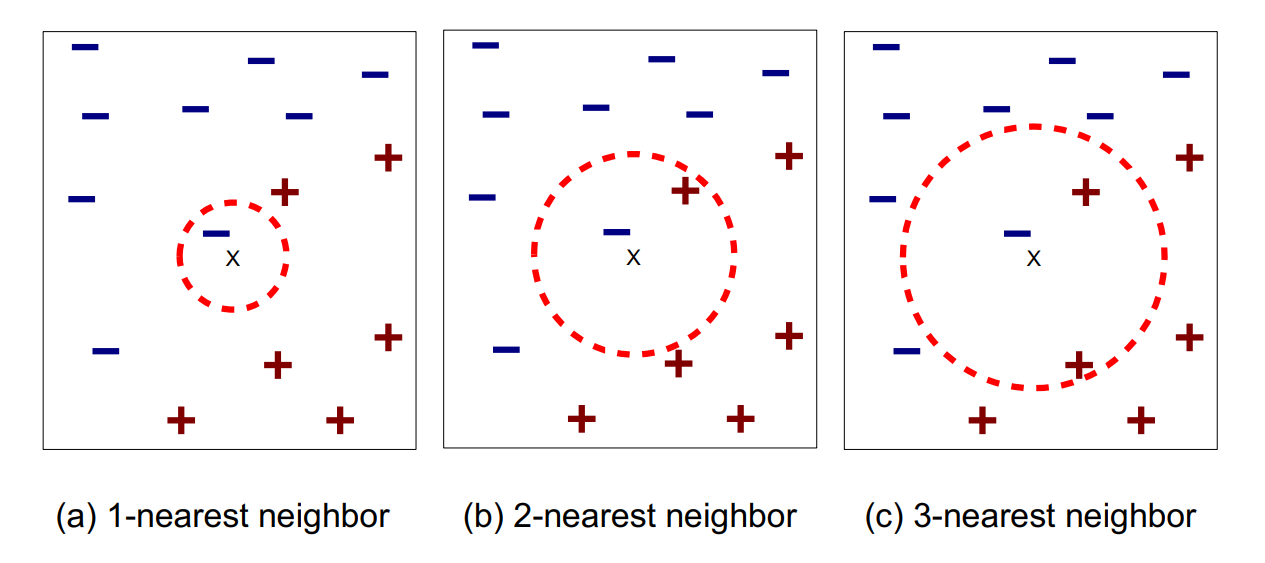
\includegraphics[width=0.97\linewidth]{im/kNNex.png}
  \caption{The $k$-nearest neighbors of an unclassified record $x$ (center) with $k$ smallest distances to $x$.}
  \label{fig:kNN1}
\end{figure}

Choosing an appropriate value for $k$ is critical for the model to predict optimally. If $k$ is chosen to be large the neighbors may contain other classes, whereas if $k$ is chosen to be small the model may become too sensitive to outliers and noise. \autocite{patternrecognition} Since we are concerned with two classes, we have to choose $k$ to be an odd number. For $k = 1$, a \textit{Voronoi partition} occurs, an example of which is shown in Figure 3.6, wherein the regions are defined by: \autocite{introdatamining}
\begin{equation}
    R_i = \{ x : d(x, x_i) < d(x,x_j), i \neq j \}
\end{equation}

\begin{figure}[h!]
  \centering
  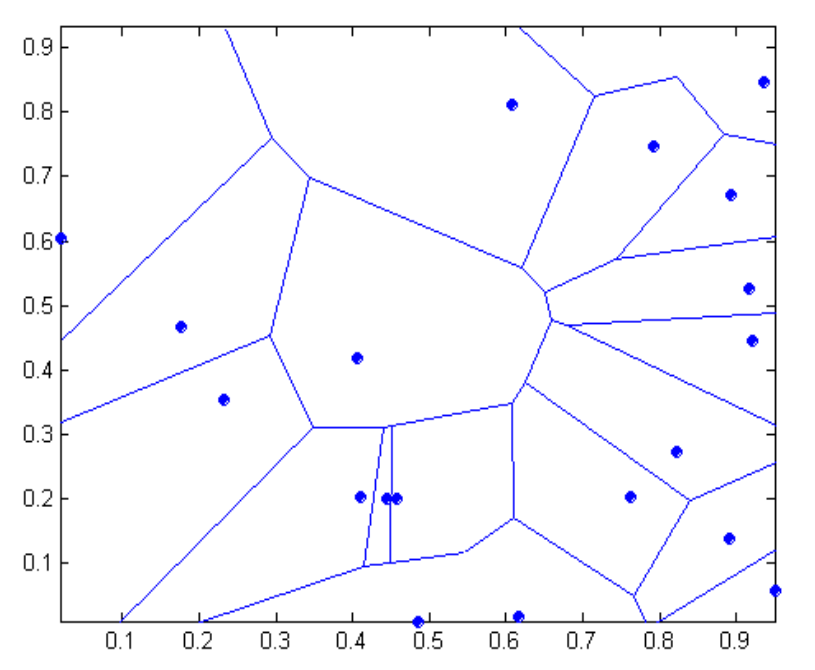
\includegraphics[width=0.5\linewidth]{im/1NNVoronoi.png}
  \caption{Voronai diagram representing regions $R_i$ from a \textit{k}NN where $k=1$.}
  \label{fig:1NN}
\end{figure}

\newpage
In any case, distances $d$ from a point are calculated using the Euclidean distance formula and this can be used to calculate a weight factor, $w$, to give greater significance to classes closer to the point:

\begin{equation}
    d(p,q) = \sqrt{\sum_i(p_i - q_i)^2}
\end{equation}
\begin{equation}
    w = \frac{1}{d^2}
\end{equation}

The main drawback of the \textit{k}NN algorithm is the complexity and computational expense of searching for the nearest neighbors. Furthermore, since the algorithm exclusively uses the training data it was provided in order to classify, it is essential that the dataset accurately represents real-world phenomenon. We should be aware of this since the data we have used was generated from the Monte Carlo program CORSIKA. Especially for this classification method, the model will only be as accurate as our computer-generated dataset. As such, this model may have trouble classifying real data from an IACT. However, its use of local information and ability to create arbitrary boundaries makes it a useful model to consider and understand the data.

\section{Logistic Regression}

Logistic Regression is originally a statistical method that can be used to classify data using probabilities derived from a linear combination of features. The resulting probability indicates how likely a new instance of data belongs to a certain class. Naturally, the sum of the probabilities for each of the individual classes is one. Although our logistic regression algorithm models a binary dependent variable, it may also be extended in order to be able to predict the likelihoods of more classes. Multiple variations of this method exist, though Mathematica uses it through the following means.

Given a linear combination of numerical features, $x = \{x_1,x_2,\dots, x_n\}$, and the parameters for class $k$ represented by $\theta^{(k)} = \{\theta_1, \theta_2,\dots, \theta_m\}$, the logistic regression algorithm can model the log probabilities of each class which is given such that: 
\begin{equation}
        \log \left( P(\text{class}=k|x) \right) \propto x.\theta^{(k)}
\end{equation}

The parameter matrix denoted as $\theta = \{\theta^{(1)}, \theta^{(2)},\dots, \theta^{(n)}\}$ can then be approximated by minimizing the loss function, which is given by the equation:
\begin{equation}
\sum_{i=1}^m-\log(P_{\theta}(\text{class}=y_i|x_i))+\lambda_1 \sum_{i=1}^n |\theta_i|+\frac{\lambda_2}{2} \sum_{i=1}^n\theta_i^2    
\end{equation}

The optimization methods available in Mathematica for this particular classification method include the limited memory Broyden-Fletcher-Goldfarb-Shanno algorithm, the stochastic gradient descent method, and the Newton method. Although logistic regression models are relatively easy to understand, they are relatively computational and mathematical in nature.

\chapter{Approach}

This chapter describes how the classification models may be constructed.

\section{Use of Mathematica}

To come to a conclusion about which of the five methods is best for the data of an IACT, we must construct models with the data. This was done using Wolfram Mathematica version 12.0.0.0. The program Mathematica contains many advanced computational functions, such as \texttt{Classify}. This function allows the simple construction of predictive models using any of the five methods described in the previous section. There are also additional methods available for the function, but we will focus our interest in the five described. Mathematica was chosen for its large repertoire of built-in, high-level, technical algorithms as well as for its ease of use. 

Use of the same program for the creation of all five classification models will lead to homogeneity with regard to the internal dynamics of the model other than the \texttt{Method} used. The models may be further improved by the implementation of \textit{cross-validation}, in which each model is trained multiple times. This helps avoid abnormal cases of the model. However, this was not implemented in our code. Additionally, we used \texttt{Import} instead of \texttt{SemanticImport} due to trouble with the latter function.

\newpage

\section{Prototype code}
\begin{verbatim}
Clear["Global`*"];
mydat = Dataset[
   Import["X:\\My Desktop\\thesis stuff\\magic04.json",
   "RawJSON"] (* Import file here *) ];
classifierSet = RandomSample[mydat];
trainingFraction = 0.35;
ntrain = Round[trainingFraction Length[classifierSet]];
trainingSet = classifierSet[1 ;; ntrain];
testSet = classifierSet[ntrain ;; Length[classifierSet]];

cmodel = Classify[
   trainingSet -> "class",
   PerformanceGoal -> "Quality",
   Method -> "NeuralNetwork", (* Select a method from:
        {"NeuralNetwork", "DecisionTree", "RandomForest", 
        "NearestNeighbors", "LogisticRegression"} *)
   ValidationSet -> None,
   TrainingProgressReporting -> "Panel"
   ];

Print@ClassifierInformation[cmodel] 
Print@ClassifierMeasurements[cmodel, testSet -> "class",
    "ConfusionMatrixPlot"]
Print@ClassifierMeasurements[cmodel, testSet -> "class",
    "ROCCurve"]
\end{verbatim}

\chapter{Implementation}

This chapter deals with the properties of the generated models. In that regard, we compare the models to see which ones perform optimally with our dataset.

\section{Classifier information}

The code given in Section 4.2 was run five times, and each time some properties of the generated model was saved. The \texttt{Method} parameter of the \texttt{Classify} function was changed to the desired machine learning method at each of these five iterations. During the implementation process we experienced difficulty in implementing the \texttt{SemanticImport} function. Thus the dataset was converted from a \texttt{.data} file into a raw \texttt{.json} file. This was then imported into Mathematica using the \texttt{Import} function. It was decided, somewhat arbitrarily, that 35\% of the dataset would be used to train each classifier, and the rest would be used for testing. This resulted in a training set of 6657 events or instances. The rest of the dataset became the test set. As mentioned earlier, cross validation was not implemented but remains an option for further improvement. The general information of the classifier models are given in the following pages.

\begin{figure}[p]
  \centering
  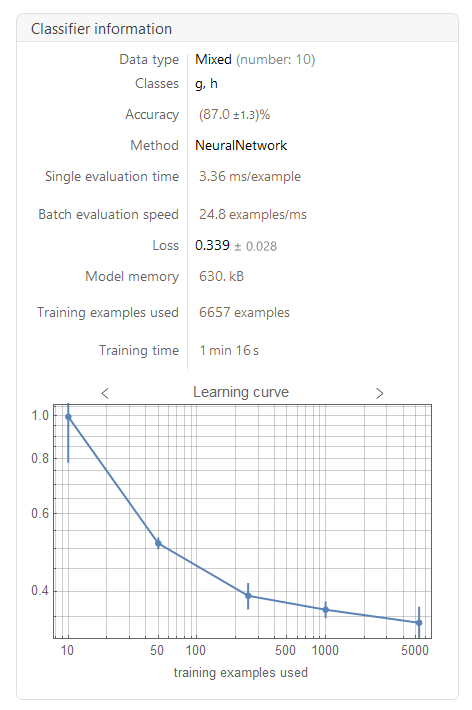
\includegraphics[scale=0.75]{models/nn1.png}
  \caption{Classifier information of the Neural Network model.}
\end{figure}

\begin{figure}[p]
  \centering
  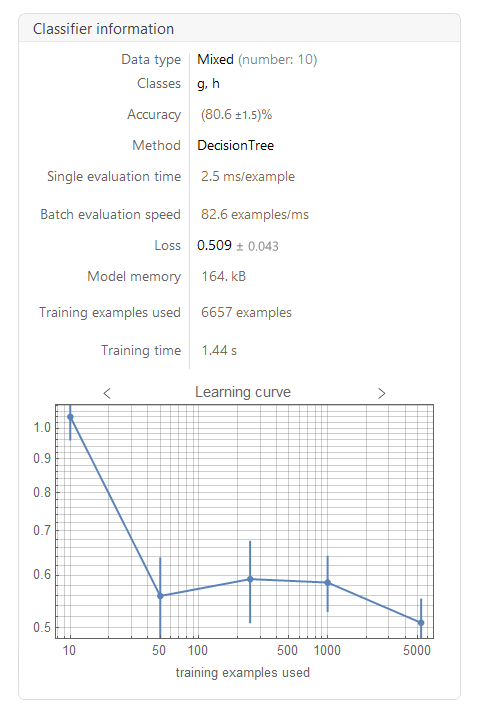
\includegraphics[scale=0.75]{models/dt1.png}
  \caption{Classifier information of the Decision Tree model.}
\end{figure}

\begin{figure}[p]
  \centering
  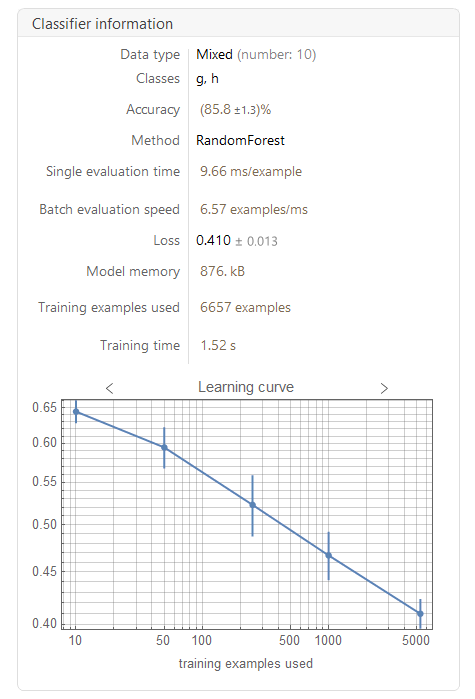
\includegraphics[scale=0.75]{models/rf1.png}
  \caption{Classifier information of the Random Forest model.}
\end{figure}

\begin{figure}[p]
  \centering
  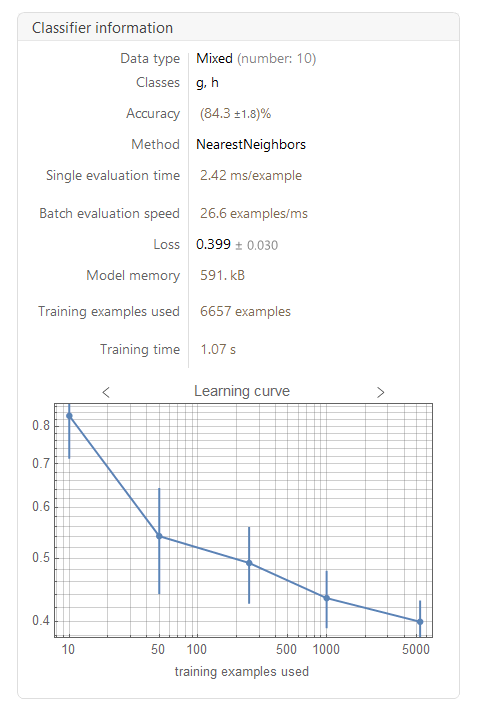
\includegraphics[scale=0.75]{models/knn1.png}
  \caption{Classifier information of the Nearest Neighbors model.}
\end{figure}

\begin{figure}[p]
  \centering
  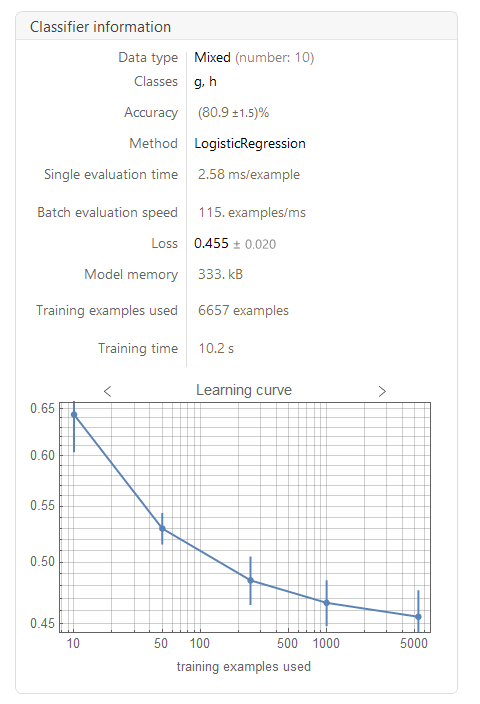
\includegraphics[scale=0.75]{models/lr1.png}
  \caption{Classifier information of the Logistic Regression model.}
\end{figure}

\newpage

\section{F-measure}

The Confusion Matrix is an ideal tool for determining the effectiveness of our models. Our models predict the likelihood of an instance being in one of two classes. Since the models are to detect the presence of a gamma ray, the gamma (g) class is our true value and the hadron (h) class is our false value. In our case, predicting a gamma ray when the instance is a hadron is worse than predicting a hadron when the instance is a gamma ray. Thus a False Positive (Type I Error) should be penalized harder than a False Negative (Type II Error). Our confusion matrices list the predicted and actual values under a classification method as follows:

\begin{figure}[h!]
    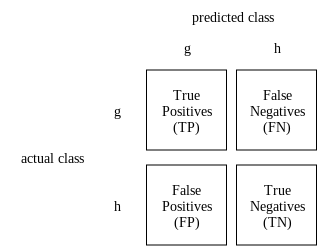
\includegraphics[scale=0.9]{im/conmatexform.png}
    \caption{Format of our confusion matrices.}
    \label{fig:conmatex}
\end{figure}

A confusion matrix gives us parameters with which we can evaluate how well the models performed. We will do so firstly with the use of the \textit{F-measure} or \textit{F-value}. This will be calculated for our data with the following steps.

\newpage

The \textit{precision} is the fraction of correctly identified gamma rays and all the instances where the model predicted a gamma ray:
\begin{equation}
    \text{Precision} = \frac{\text{TP}}{\text{TP}+\text{FP}}
\end{equation}

The \textit{recall}, or true positive rate, is the fraction of correctly identified gamma rays and all the instances where the signal was truly a gamma ray: 
\begin{equation}
    \text{Recall} = \frac{\text{TP}}{\text{TP}+\text{FN}}
\end{equation}

The \textit{F-measure} is the harmonic mean of the precision and recall:
\begin{equation}
    F = 2 \times \frac{\text{Precision} \times \text{Recall}}{\text{Precision} + \text{Recall}}
\end{equation}

The values for each of these properties is tabulated below:

\begin{center}
    \begin{table}[h!]
    \centering
        \renewcommand{\arraystretch}{2}
        \begin{tabular}{ p{4cm}  p{2cm}  p{2cm}  p{2cm} }
        \textit{Method} & \textit{Precision} & \textit{Recall} & \textit{F-measure} \\
            Neural Network & 0.865888  & 0.923047 & \textbf{0.893554} \\
            Decision Trees & 0.851266 & 0.845330 & \textbf{0.848287} \\
            Random Forest & 0.867894 & 0.942352 & \textbf{0.903592}\\
            Nearest Neighbors & 0.804898 & 0.955754 & \textbf{0.873863} \\
            Logistic Regression & 0.803349 & 0.903793 & \textbf{0.850616} \\
        \end{tabular}
        \caption{\label{tab:models} Evaluation properties of the models.}
    \end{table}
\end{center}

\begin{figure}[p!]
\centering
\begin{tabular}{cccc}
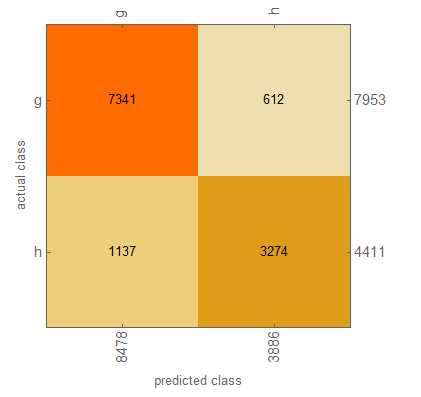
\includegraphics[width=0.43\textwidth]{models/nn2.png} &
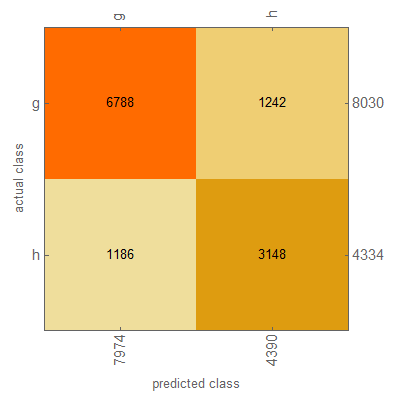
\includegraphics[width=0.43\textwidth]{models/dt2.png} \\
\text{(a) Neural Network}  & \text{(b) Decision Trees}  \\[6pt]
\end{tabular}
\begin{tabular}{cccc}
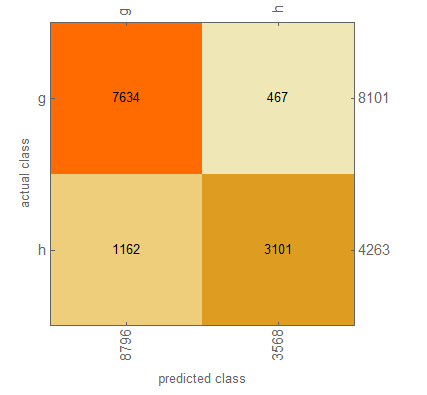
\includegraphics[width=0.43\textwidth]{models/rf2.png} &
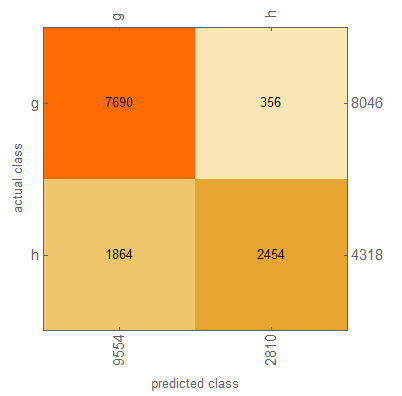
\includegraphics[width=0.43\textwidth]{models/knn2.png} \\
\text{(c) Random Forest}  & \text{(d) Nearest Neighbors}  \\[6pt]
\end{tabular}
\begin{tabular}{cccc}
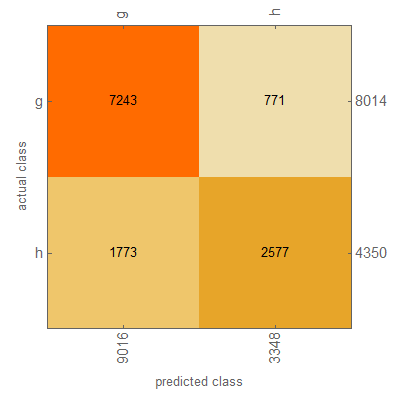
\includegraphics[width=0.42\textwidth]{models/lr2.png} \\
\text{(e) Logistic Regression}  \\[6pt]
\end{tabular}
\caption{Confusion matrices of the five models.}
\label{fig:conmats}
\end{figure}

\newpage

\section{ROC curve}

A Receiver (sometimes Relative) Operating Characteristic (ROC) curve is a graphical plot of the recall (true positive rate) versus the false positive rate. This is also a useful means of validating our models. ROC curves summarize the confusion matrices that each of the threshold parameters of the model produced. ROC curves can be used to select the best threshold for a given model, but they can also be used to judge which models perform better than others. The greater the area under the curve (AUC), the better the model is at predicting the correct class. The area is represented by a blue shading. An example ROC curve, with a varied confusion matrix form, is shown below. \autocite{rocex} The false positive rate (FPR) is given by the equation:
\begin{equation}
    \text{FPR} = \frac{\text{FP}}{\text{FP}+\text{TN}}
\end{equation}

\begin{figure}[h!]
    \centering
    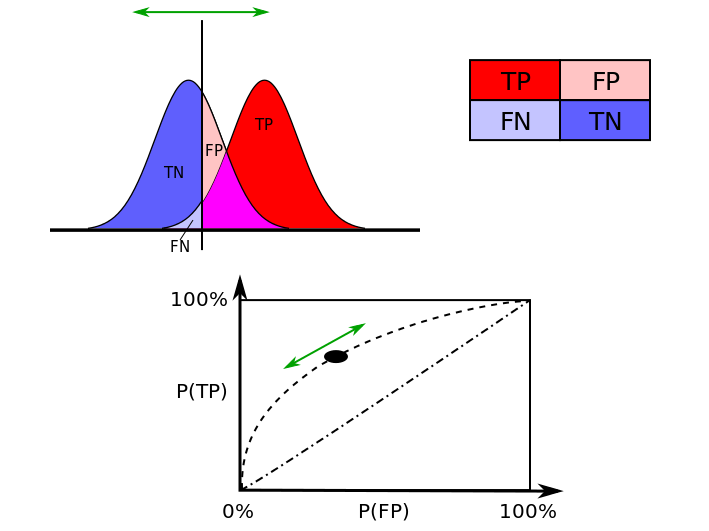
\includegraphics[scale=0.34]{im/ROCcurves.png}
    \caption{An example ROC curve.}
    \label{fig:rocex}
\end{figure}

\begin{figure}[p]
  \centering
  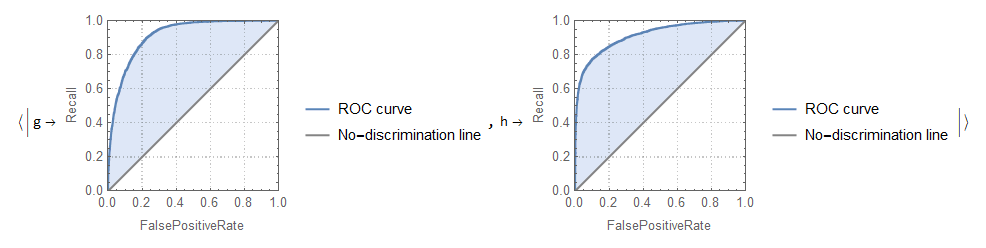
\includegraphics[width=0.9\textwidth]{models/nn3.png}
  \text{(a) Neural Network}
  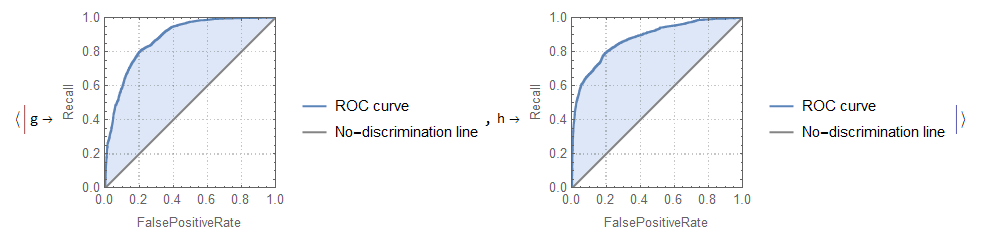
\includegraphics[width=0.9\textwidth]{models/dt3.png}
  \text{(b) Decision Trees}
  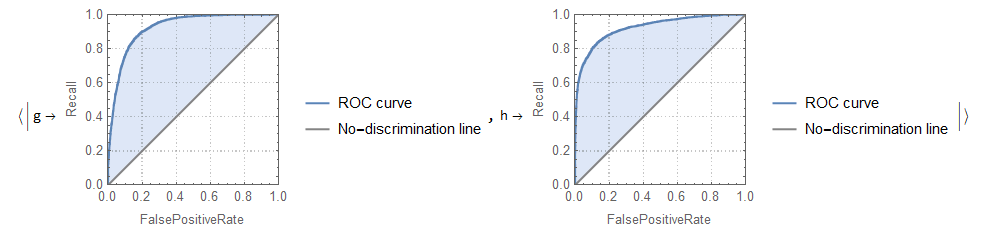
\includegraphics[width=0.9\textwidth]{models/rf3.png}
  \text{(c) Random Forest}
  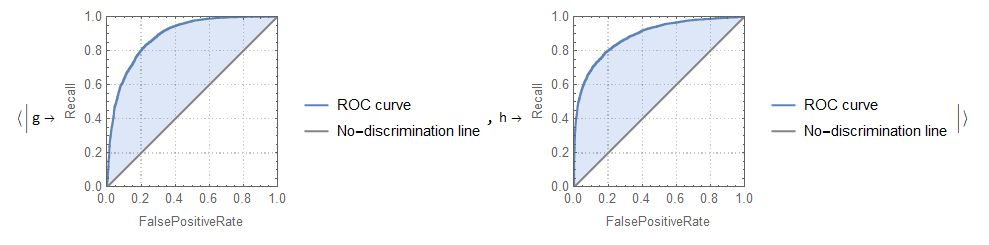
\includegraphics[width=0.9\textwidth]{models/knn3.png}
  \text{(d) Nearest Neighbors}
  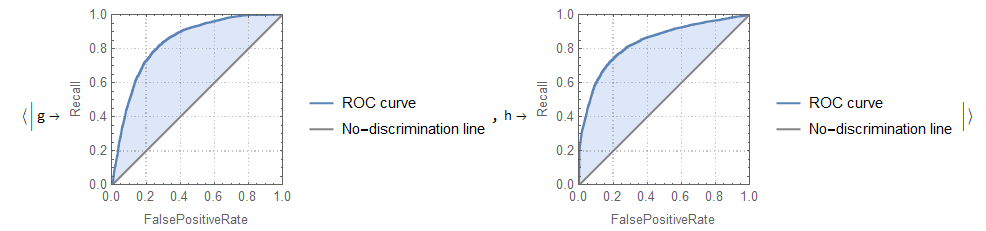
\includegraphics[width=0.9\textwidth]{models/lr3.png}
  \text{(e) Logistic Regression}
  \caption{ROC curves of the five model.}
\end{figure}

\chapter{Evaluation}

\section{Which is the best method?}

Interestingly enough, all our generated models performed well, with F-values between approximately 0.85 and 0.90. The two methods with the highest F-values as well as the greatest areas under the ROC curve were the Neural Network and Random Forest models. These were generally on par with each other. The Neural Network model had better accuracy, fewer Type I errors, and faster evaluation times than the Random Forest model. Thus it is a viable model for our case. However, the Random Forest algorithm had a slightly higher F-value (manual cross-validation was done to confirm this was generally true) and required significantly less training time than the Neural Network model. Additionally, a Random Forest model is relatively more explicit in generating classification rules, easier to work with, and better at handling missing data. Thus we are inclined to giving the Random Forest algorithm the title of best machine learning method for use with an IACT. Interestingly, the Decision Trees model, which has ties with the Random Forest model, performed the worst. The second to worst was the Logistic Regression model. The performance of the Nearest Neighbors model was just shy of the Neural Network and Random Forest models. Note that here the F-values mirrored the area under the ROC curves. Regardless, it should be reiterated that all the models performed decently and have the potential of being made more effective.

\section{Testing with adversarial data}

In order to test that the models were indeed making sense of the data, the Random Forest algorithm was made to classify randomly generated data. The new \enquote{adversarial} test dataset contained random real numbers between 0 and 1 for each of the attributes in the dataset. So this dataset should make no sense when looked at as an IACT observation. Running the model on this new meaningless dataset gave us an accuracy of 49.875\%, which is very close to 50\%. Given two options, the probability that the model guesses and gets the answer right by chance is \textonehalf, or 50\%. This implies \enquote{no discrimination}, and that the models did not mistakenly think that the meaningless dataset showed properties of an IACT observation. The ROC curve for the gamma class also indicates that the classifier understood that the data was randomly generated. This is reproduced below:

\begin{figure}[h!]
    \centering
    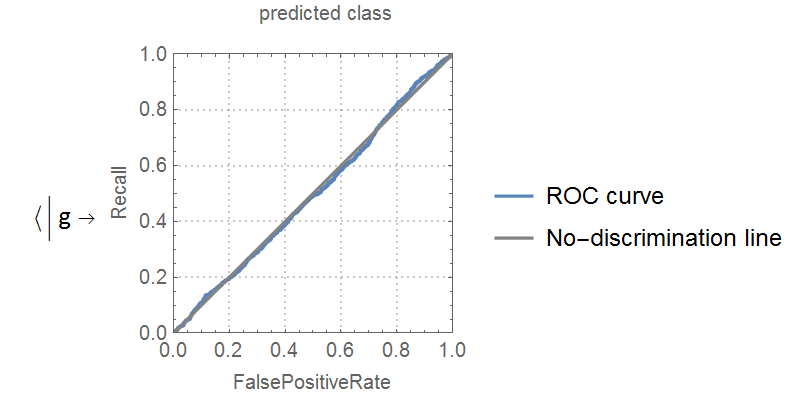
\includegraphics[scale=0.42]{im/testonrf.png}
    \caption{The \enquote{g} class ROC curve of the RF model using adversarial data.}
    \label{fig:testrf}
\end{figure}

\newpage

\section{Limitations}

The models that were constructed provide a decent classification of the dataset in question. Unfortunately, models such as this are prone to becoming a case of \enquote{garbage in, garbage out}. In cases such as ours, there is not a lot that can be done to objectively check the quality of the sample data, namely the accuracy of the class labels. Although the two methods that performed best in our exercise did classify the data quite accurately, their internal architectures leave much to be desired when it comes to actually understanding how the classes were distinguished from each other. Moreover, the performance of these two models did not differ significantly, so choosing between them may be trivial. Machine learning methods such as decision trees, nearest neighbors, and logistic regression -- albeit a little worse off at classification accuracy -- create algorithms that are better comprehensible to humans. This criterion is important because we ourselves would like to know how distinctions were made and if the discrimination rules make sense. Understandability depends on the structure of the classification rules that the model creates. Sometimes, the optimal use of machine learning is restricted due to factors such as available computational time and knowledge of the field. This sometimes makes it difficult to apply models such as these into the real world.

%\newpage

\section{Outlook}

With the advent of machine learning, many processes that would have been tedious otherwise can now be performed with minimum human effort. As computational capability increases and new techniques are discovered to make classification models even more accurate, new possibilities for data manipulation also open up. The automation of computational processes will undoubtedly improve the speed at which new interpretations can be made. The analysis of data with the help of machine learning has the potential of greatly increasing our understanding of the internal mechanisms of systems. Since the classifiers can model data in ways that humans might not be able to imagine, they have the potential of allowing us to discover previously hidden patterns within the data. Different machine learning methods provide different views of data and how data may be classified. In that regard, even the models that were constructed here can potentially be improved by techniques such as cross-validation, using more training data, and other optimization strategies. For further research, it would be interesting to implement both the neural network and random forest models into the telescope since they performed at nearly the same level. Some features of one of these models could make it much better than the other when implemented into MAGIC. It should go without saying that increased knowledge in this field will pave the way to a better understanding of natural phenomena. In our case, the detection of gamma rays can be done more reliably. Machine learning can be used as a powerful tool to help handle the explosion of available data in Astronomy.

\chapter{Conclusions}

%connecting data to real world and connecting model to the real world

% head meets tail

In this paper, we aimed to evaluate which machine learning methods are optimal for the classification of data from an IACT. To answer this question, we constructed five machine learning classifiers using the same programming environment in Wolfram Mathematica. Our observations indicated that all of the machine learning methods performed well as a binary classifier, distinguishing gamma ray events from noise. However, we noticed that \textbf{the Random Forest classifier performed best}, having the greatest area under the ROC curve and the highest F-measure, as well as requiring significantly less training time compared to the second to best model; though the best two performed almost equally well. This classification method works by aggregating the answers of multiple Decision Trees.

In answering the research question, we have demonstrated the usefulness of machine learning as well as how it is not difficult to work with anymore. Interestingly, we have also showed that most of our chosen classification methods perform decently with our dataset. The increasing amounts of Astronomy data, coupled with the development of even better technologies and the increasing accessibility to machine learning methods, indicates that there will be much more activity in this area of knowledge. Finally, we have created a sort of manual to bridge any gap between these different disciplines that have the potential to benefit greatly from one another.
 
 \newpage
\addcontentsline{toc}{chapter}{Bibliography}
 
\printbibliography
\end{document}